\subsubsection{Tutor Session \& Progress Management}
\begin{figure}[H]
    \centering
    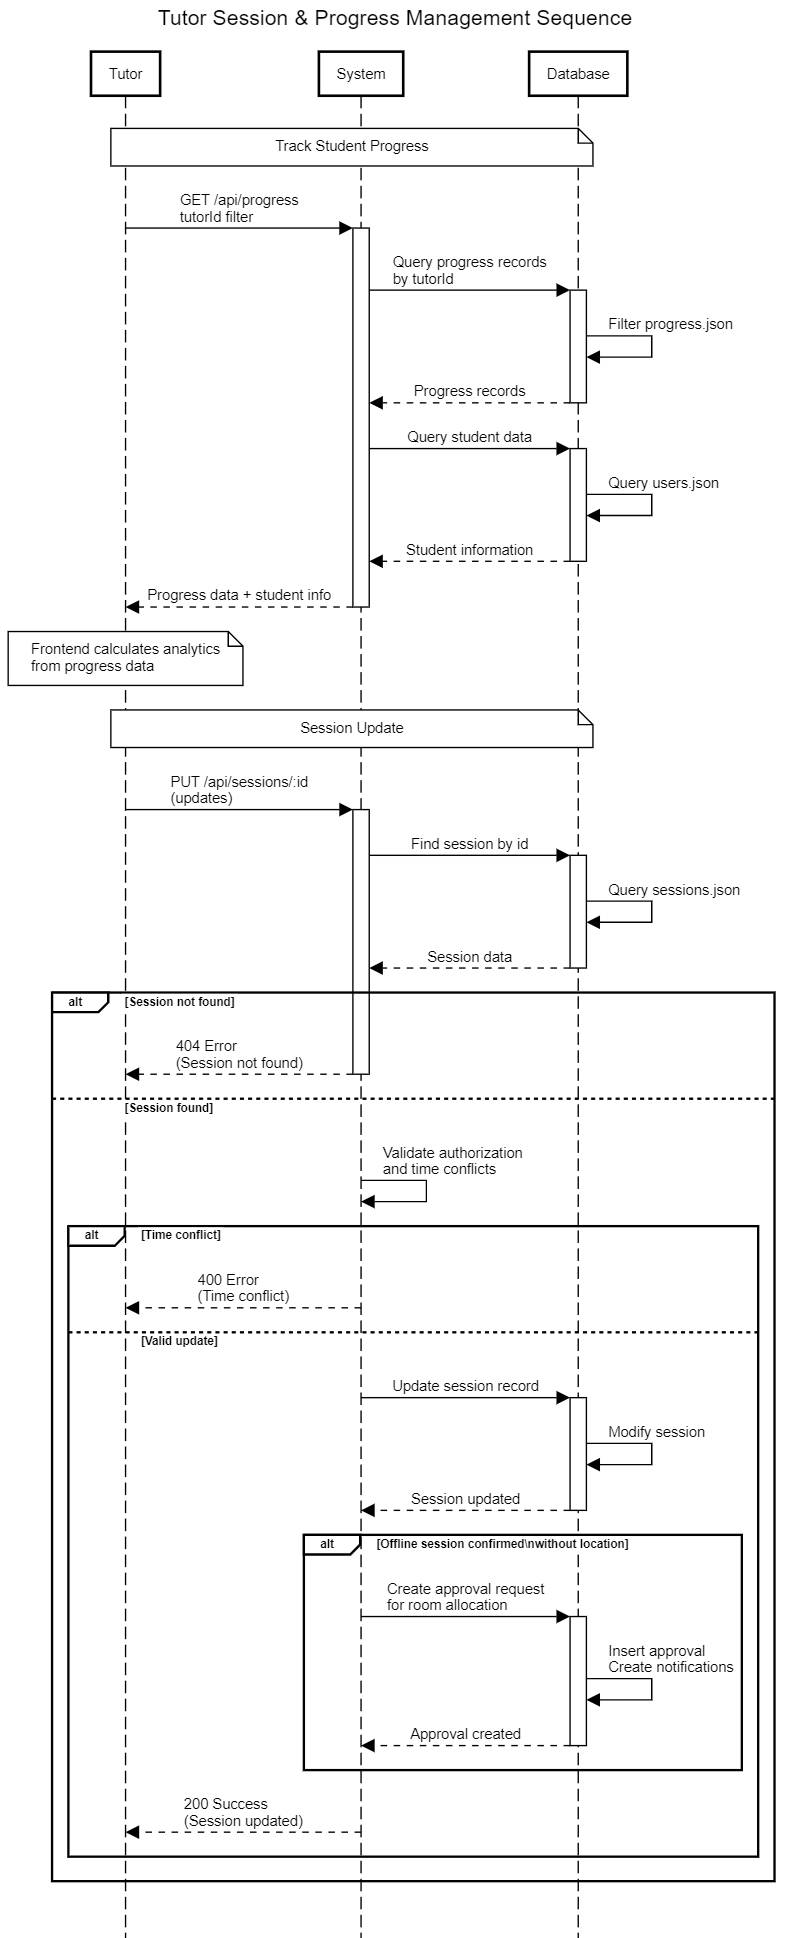
\includegraphics[width=0.5\textwidth]{graphics/chapter3/tutor/session_progress.png}
    \caption{Sequence diagram of Tutor Session \& Progress Management}
    \label{fig:session_progress_management}
\end{figure}

\newpage
\noindent \textbf{Description} \\ 

\textbf{Actors:} Tutor, System, Database

\textbf{Flow 1: Track Student Progress}

\begin{enumerate}
    \item Tutor requests progress data from System (GET /api/progress with tutorId filter)
    \item System queries Database for progress records and student information
    \item Database returns progress data and student info to System
    \item System returns data to Tutor
    \item Frontend calculates analytics from progress data
\end{enumerate}

\textbf{Flow 2: Session Update}

\begin{enumerate}
    \item Tutor sends session update request to System (PUT /api/sessions/:id)
    \item System validates authorization and checks for time conflicts
    \item System updates session record in Database
    \item If offline session confirmed without location, System creates approval request for room allocation
    \item System returns success response to Tutor
\end{enumerate}




